\documentclass[xcolor=svgnames]{beamer}
\usepackage[utf8]{inputenc}
\usepackage[T1]{fontenc}
\usepackage{xcolor}
\usepackage{booktabs}
\usepackage{amsmath}
\usepackage{graphicx}
\usepackage{hyperref}
\usepackage{mhchem} % Added for chemistry

\usetheme{Madrid}

% COLORS (As provided)
\definecolor{mqred}{RGB}{166, 25, 46}
\definecolor{mqdeepred}{RGB}{118, 35, 47}
\definecolor{mqgray}{RGB}{55, 58, 54}
\definecolor{mqlightgray}{RGB}{237, 235, 229}
\definecolor{mqmagenta}{RGB}{198, 0, 126}
\usecolortheme[named=mqred]{structure}
\setbeamercolor{title in head/foot}{bg=mqlightgray, fg=mqgray}
\setbeamercolor{author in head/foot}{bg=mqdeepred}
\setbeamercolor{page number in head/foot}{bg=mqdeepred, fg=mqlightgray}

% FOOTNOTE ARRANGEMENTS (As provided)
\makeatletter
\setbeamertemplate{footline}{
  \leavevmode%
  \hbox{%
  \begin{beamercolorbox}[wd=.5\paperwidth,ht=2.25ex,dp=1ex,center]{author in head/foot}%
    \usebeamerfont{author in head/foot}\insertshortauthor\expandafter\ifblank\expandafter{\beamer@shortinstitute}{}{~~(\insertshortinstitute)}
  \end{beamercolorbox}%
  \begin{beamercolorbox}[wd=.4\paperwidth,ht=2.25ex,dp=1ex,center]{title in head/foot}%
    \usebeamerfont{title in head/foot}\insertshorttitle
  \end{beamercolorbox}%
  \begin{beamercolorbox}[wd=.1\paperwidth,ht=2.25ex,dp=1ex,center]{page number in head/foot}%
    \usebeamerfont{page number in head/foot}\insertframenumber{} / \inserttotalframenumber
  \end{beamercolorbox}}%
  \vskip0pt%
}
\makeatother
\beamertemplatenavigationsymbolsempty

% TITLE, AUTHORS, INSTITUTE, DATE
\title[Org Chem: Mapping Reactions]{Lesson 1: Mapping the Territory}
\subtitle{Visualising Functional Group Interconversions}
\author[P. Haynes]{Mr Haynes} % Replace if needed
\institute[GHS]{Gosford High School}
\date{Module 7: Organic Chemistry}

\begin{document}

\begin{frame}
    \titlepage
\end{frame}

\begin{frame}{Outline}
    \tableofcontents
\end{frame}

\section{Introduction}
\begin{frame}{Why Map Reactions?}
    \frametitle{Introduction: Why Map Reactions?}
    \textbf{Focus Inquiry Question:} How are different classes of organic compounds interconverted through reaction pathways?
    \vspace{1em}

    \begin{itemize}
        \item \textbf{Recap Quiz:} (Teacher to ask 1-2 quick questions on recent reactions, e.g., alkene addition product, alkane substitution condition).
        \item Organic reactions don't exist in isolation – they form an \textbf{interconnected network}.
        \item Learning the connections is key to understanding organic chemistry and planning syntheses.
        \item \textbf{Today's Goal:} Learn to use a visual tool (Chord Diagram) to explore this reaction network based on what we've learned so far.
    \end{itemize}
\end{frame}

\section{The Visualisation Tool}
\begin{frame}{The Chord Diagram Tool}
    \frametitle{Understanding the Visualisation}
    This tool helps us see the "map" of organic reactions.
    \vspace{1em}
    \begin{columns}[T]
        \begin{column}{0.6\textwidth}
            \textbf{Key Features:}
            \begin{itemize}
                \item \textbf{Nodes} (Outer Segments): Represent Functional Groups (e.g., Alkane, Alkene, Alcohol).
                \item \textbf{Chords} (Inner Bands): Represent Reactions linking functional groups.
                \item \textbf{Colour Coding:} Indicates Reaction Type (Check legend/checkboxes - e.g., Addition, Substitution).
                \item \textbf{Hover/Click:} Reveals details for a specific reaction (Reagents, Conditions).
                \item \textbf{Filtering:} Checkboxes allow focusing on specific reaction types.
            \end{itemize}
        \end{column}
        \begin{column}{0.4\textwidth}
            \begin{figure}
                % Replace with a screenshot of the tool focusing on known reactions
                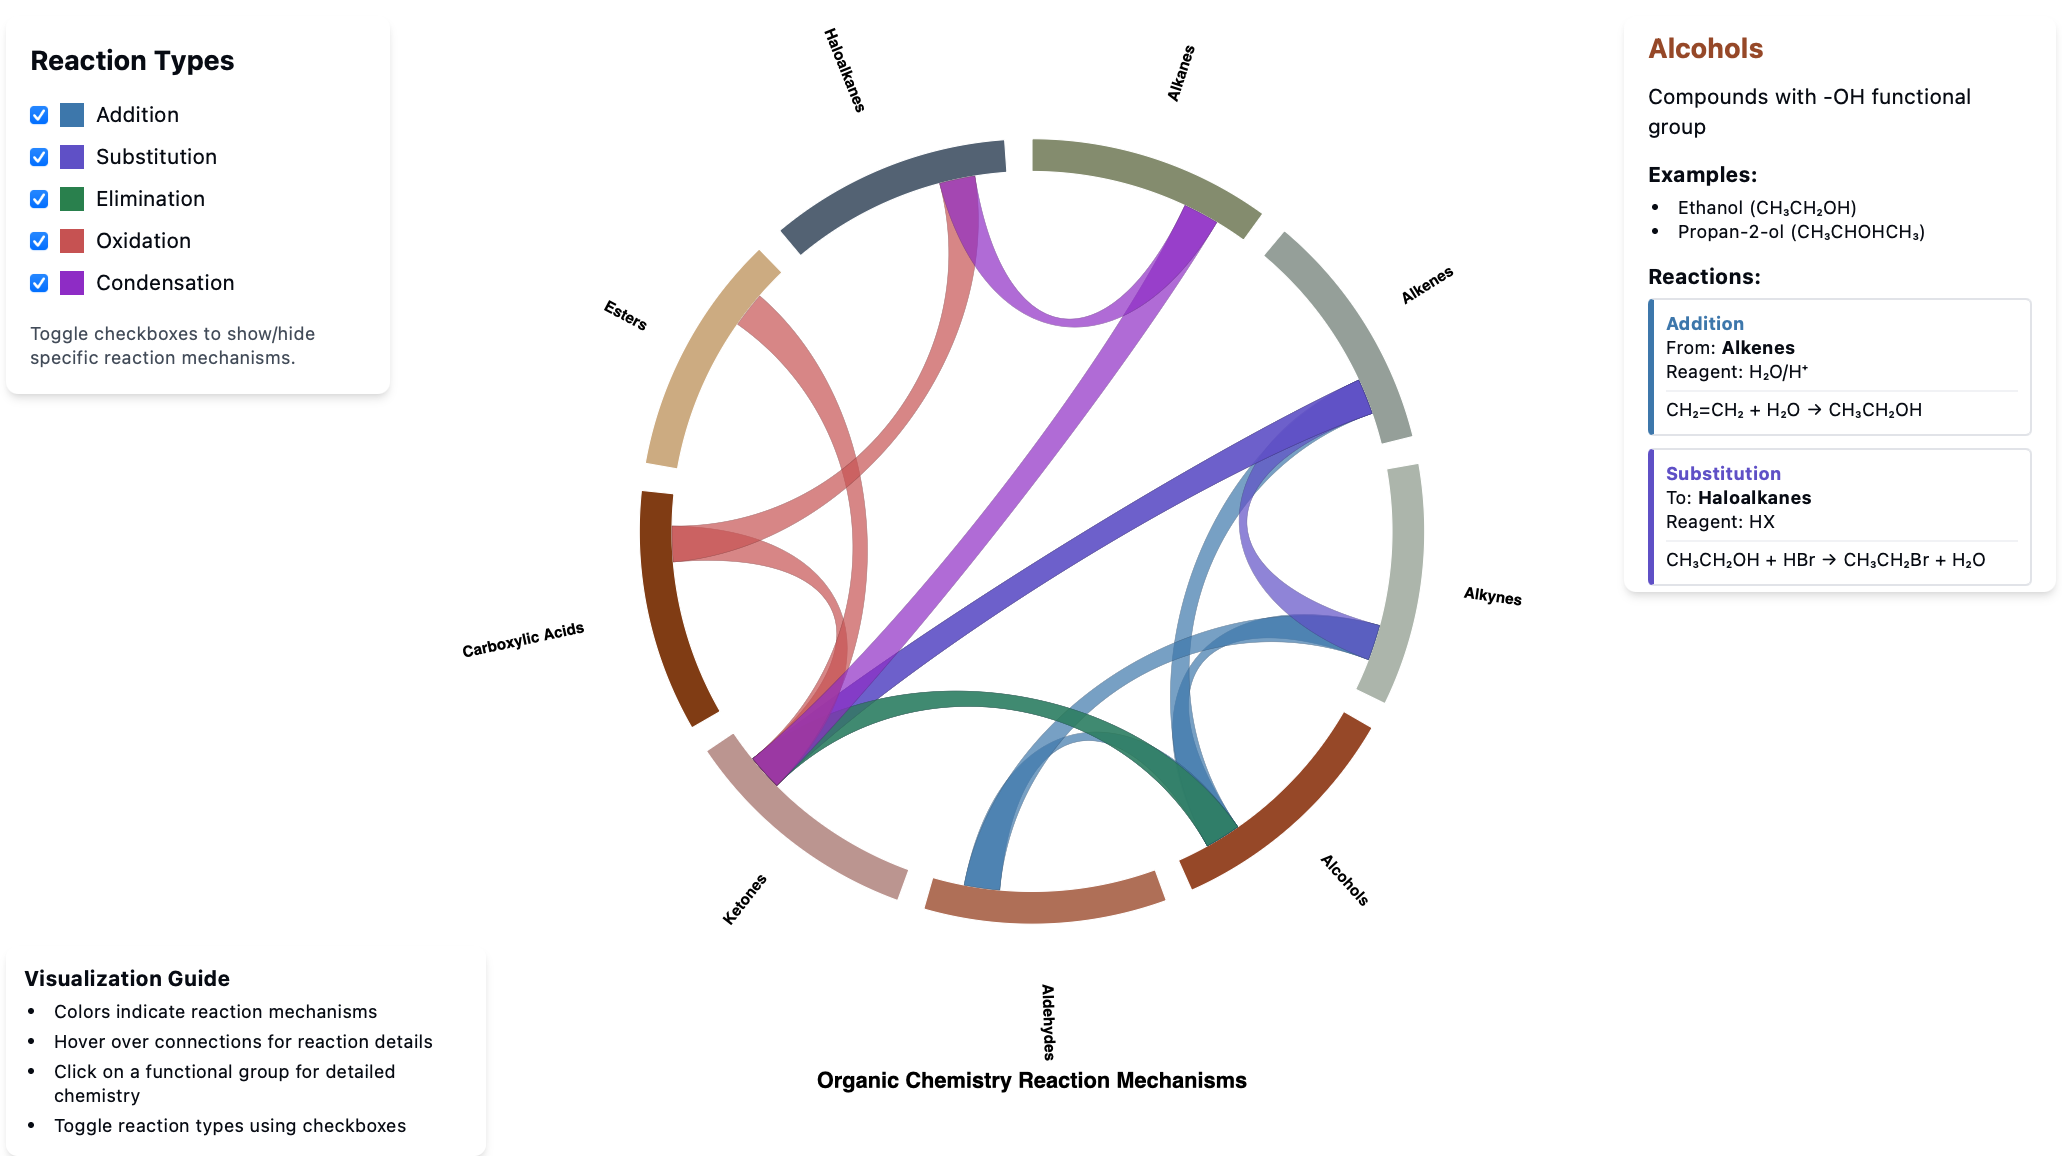
\includegraphics[width=\linewidth]{img/all-organic-chem.png}
                \caption{Chord Diagram Example}
            \end{figure}
        \end{column}
    \end{columns}
    \vspace{1em}
    \textbf{Linking Visual to Symbolic:}
    \textit{Example:} The reaction \ce{CH2=CH2 + HBr -> CH3CH2Br} would appear as a chord connecting the 'Alkene' node to the 'Haloalkane' node. Hovering reveals 'HBr'.
\end{frame}

\section{Guided Exploration}
\begin{frame}{Exploring Connections}
    \frametitle{Using the Tool for Known Reactions}
    Now, let's use the tool to map out the reactions we've already covered.
    \vspace{1em}
    \textbf{Activity Prep (Refer to Activity Sheet 1 / Worksheet 1):}
    \begin{itemize}
        \item Access the Chord Diagram tool on your device.
        \item \textbf{Your Task:} Use the tool to find the connections between Alkanes, Alkenes, Haloalkanes, and Alcohols.
        \item For each connection (reaction):
            \begin{itemize}
                \item Identify the reaction type (using colour/filter).
                \item Find the reagents/conditions (using hover).
                \item Record your findings on Worksheet 1.
            \end{itemize}
        \item \textbf{Focus:} Connecting the visual map to the reactions you already know.
    \end{itemize}
    \textit{(Teacher circulates to assist with tool usage and understanding)}
\end{frame}

\section{Summary}
\begin{frame}{Lesson 1 Summary}
    \frametitle{Mapping the Territory: Key Takeaways}
    \begin{itemize}
        \item Organic reactions form an interconnected network or "map".
        \item The Chord Diagram tool helps visualise this network:
            \begin{itemize}
                \item Nodes = Functional Groups
                \item Chords = Reactions (coloured by type)
                \item Hover = Reagents/Conditions
            \end{itemize}
        \item This tool helps organise our knowledge and see the bigger picture.
    \end{itemize}
    \vspace{1em}
    \textbf{Next Steps:}
    \begin{itemize}
        \item Complete Worksheet 1.
        \item Complete Exit Ticket (check tool interpretation).
        \item \textbf{Preview Lesson 2:} Using the map to plan short synthesis pathways (connecting reactions).
    \end{itemize}
\end{frame}

\begin{frame}
    \centering
    \textbf{Thank you!}\\ \vspace{1em} Questions?
\end{frame}

\end{document}
